% Created 2017-09-21 qui 15:46
% Intended LaTeX compiler: pdflatex
\documentclass{report}
               \pagestyle{fancy}
\usepackage[latin1]{inputenc}
\usepackage[T1]{fontenc}
\usepackage{graphicx}
\usepackage{grffile}
\usepackage{longtable}
\usepackage{wrapfig}
\usepackage{rotating}
\usepackage[normalem]{ulem}
\usepackage{amsmath}
\usepackage{textcomp}
\usepackage{amssymb}
\usepackage{capt-of}
\usepackage{hyperref}
\usepackage{paralist}
\usepackage{tcolorbox}
\usepackage[table]{xcolor}
\usepackage{lipsum}
\usepackage{caption}
\usepackage{tabu}
\usepackage[subpreambles=true]{standalone}
\usepackage{import}
\usepackage{setspace}
\usepackage{graphics}
\usepackage[linktocpage=true]{hyperref}
\usepackage{tocloft}
\usepackage{minitoc}
\usepackage[portuguese, english]{babel}
\usepackage{subfig}
\usepackage[utf8]{inputenc}
\date{}
\title{}
\hypersetup{
 pdfauthor={},
 pdftitle={},
 pdfkeywords={},
 pdfsubject={},
 pdfcreator={Emacs 25.2.1 (Org mode 9.0.9)}, 
 pdflang={English}}
\begin{document}

\thispagestyle{firstpagestyle}

\import{latex/}{side_info}

\pagestyle{plain}
  \begin{tcolorbox}[colbak=red!5!white, colframe=red!0!white]
  \large{
  \textbf{Highlights}
  \vspace{0.1cm}
  \it
    \import{latex/}{highlights}
  }
  \end{tcolorbox}
  \vspace{-0.2cm}

\setlength{\parindent}{0cm}
\setlength{\parskip}{0.1cm}

\textbf{Global Markets.} European equities are up, the S\&P future is
unchanged. The Mexican peso, however is down by 0.2\% against the USD,
and the yield of the 10 years Treasury is up to 2.27\%. Commodities:
oil is down 0.3\% to USD50.5, steel is down 0.4\% and soy prices is
climbing about 0.7\%.

\textbf{Local News}. \textbf{The second charge against Mr. Temer should indeed go to
the Lower House}, as confirmed yesterday by the Supreme Court. In
fact, according to the Estadao, the Speaker of the Lower would have
stated he is planned to get the whole done and over by before the
October 12th holiday. 

That said, the media outlet Brodacast reports Mr. Rodrigo Maia's
discontentment with PMDB, which has sponsored the entrance of the
Minister of Energy to PMDB rather than the DEM, Mr. Maia's
party. Therefore, it remains to be seen whether this affair will
interfere in the expedience of how the charge will be handled.

In the meantime, the Lower House has given an extra step to approve
\textbf{the political reform}. It started to vote, in a second round, the
constitutional amendment on election coalitions and minimum voting
thresholds, which will have to continue on next week prior to send the bill
to the Upper House, where it faces the October 7th deadline. 

Also next week, the Lower House has another daunting task: vote the
constitutional amendment on election funding, which faces the same
deadline.

\textbf{On the fiscal front}, the Refis is giving the government an extra
headache. According to the O Valor, The Ministry of Finance is no
longer interest in approving it, since, reportedly, revenues have been
quite good so far. However, Congress would be already counting on
these benefits and dissatisfaction is growing ahead of the vote of the
second charge against Temer.

On the economic front, newspaper conveys several information about
\textbf{privatizations} to come. As \emph{per} O Valor, the government is now
studying in more in-depth the Eletrobras' case, which it has now
floated the idea of privatization the mail services.

\textbf{Agenda - Highlights}: \uline{Brazil}: BC's inflation report and mid-term
CPI. \uline{US}: jobless claims.


\rowcolors{2}{grey!15}{white}
\vspace{-0.5cm}

\begin{center}
\begin{tabular}{rlllll}
\textbf{Time} & \textbf{Country} & \textbf{Indicator} & \textbf{Period} & \textbf{Forecast} & \textbf{Impact}\\
\hline
08:00:00 & BZ & Inflation Report & Sep & - & High\\
09:00:00 & BZ & IPC-15 & Sep & 0,13\% mom & High\\
09:30:00 & US & Initial Jobless Claims & Sep 16 & 302 k & Low\\
11:00:00 & US & Leading index & Aug & 0,3\% mom & Low\\
16:30:00 & BZ & Jobs Creation & Aug & 60 k & Medium\\
\end{tabular}
\end{center}


\textbf{Bottom Line}. Global markets look a bit counter productive, while
local news look neutral.  Watch out for CB's inflation report and
mid-term inflation.

\newpage

\section{Brazilian Bonds}
\label{sec:org5e5b2cb}


\begin{center}
\textbf{NTNF} \\
\vspace{0.1cm}
\import{latex/}{NTN-F}
\end{center}
\vspace{0.5cm}

\begin{center}
\textbf{LTN} \\
 \vspace{0.1cm}
\import{latex/}{LTN}
\vspace{0.5cm}
\end{center}

\begin{center}
   \textbf{NTN-B} \\
\vspace{0.1cm}
       \import{latex/}{NTN-B}
       \vspace{0.1cm}
     \end{center}
     \newpage



\begin{center}
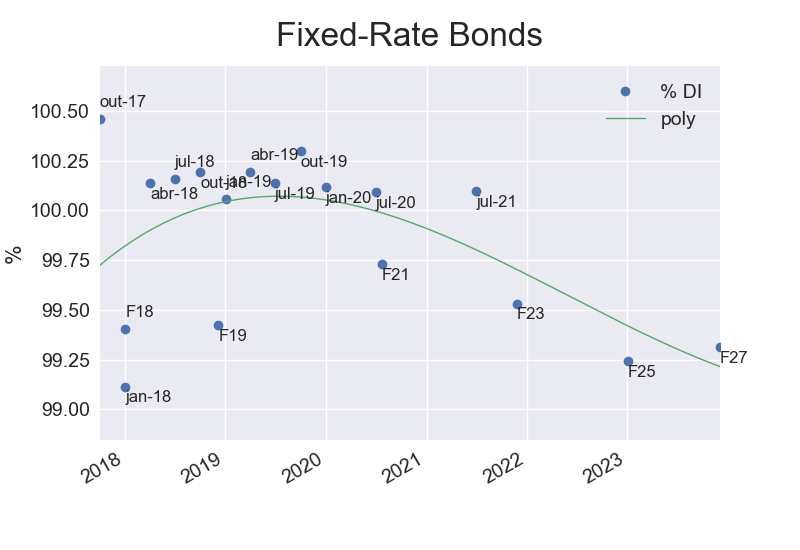
\includegraphics[width=16.0cm]{charts/fixed.png}
\end{center}

\begin{center}
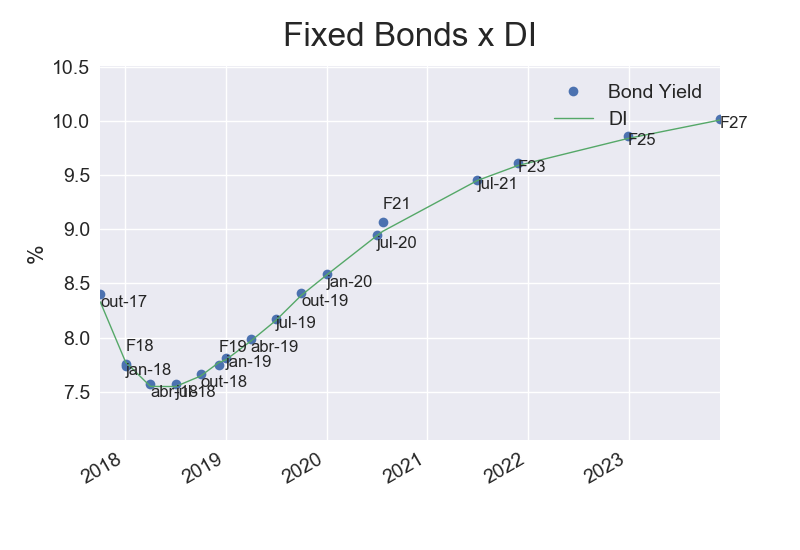
\includegraphics[width=16.0cm]{charts/fixed_di.png}
\end{center}

\begin{center}
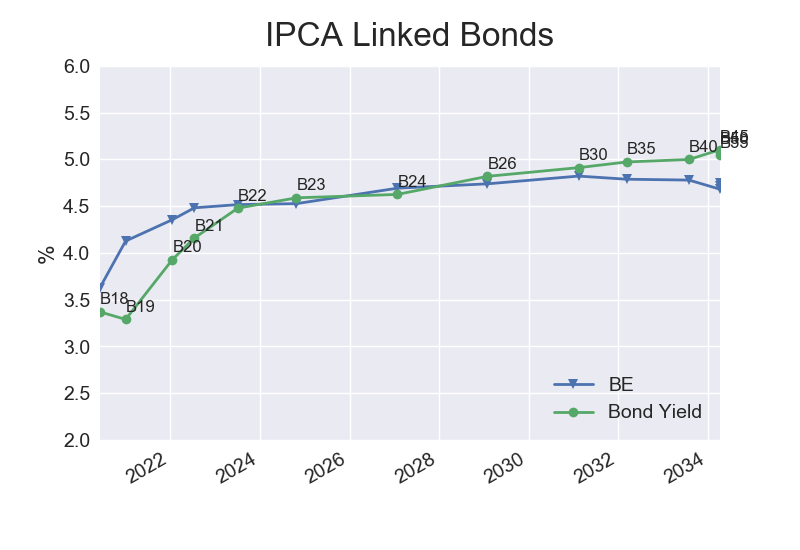
\includegraphics[width=16.0cm]{charts/ntnb.png}
\end{center}


\section{DI - Open Interest}
\label{sec:org71c6115}

  \begin{center}
    \import{latex/}{OpenInterest}
  \end{center}
\newpage

\vspace{3.0cm}
  \begin{center}
    \import{latex/}{DIContracts}
  \end{center}
\newpage


\section{DI - DV01 Table}
\label{sec:orgc699158}

  \begin{center}
    \import{latex/}{DIs}
  \end{center}
\newpage


\section{NTNB FRAs}
\label{sec:org89b3a29}


\begin{center}
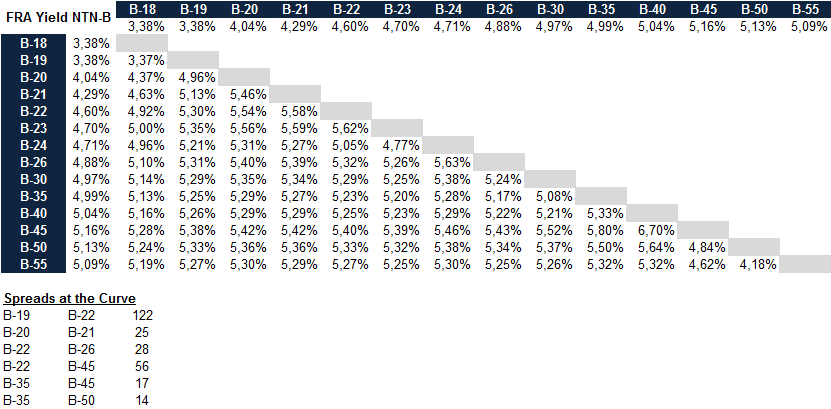
\includegraphics[angle=90,width=10.5cm]{images/FRA_NTNB.png}
\end{center}

\newpage


\section{DI FRAs}
\label{sec:orgf3cc546}
\begin{center}
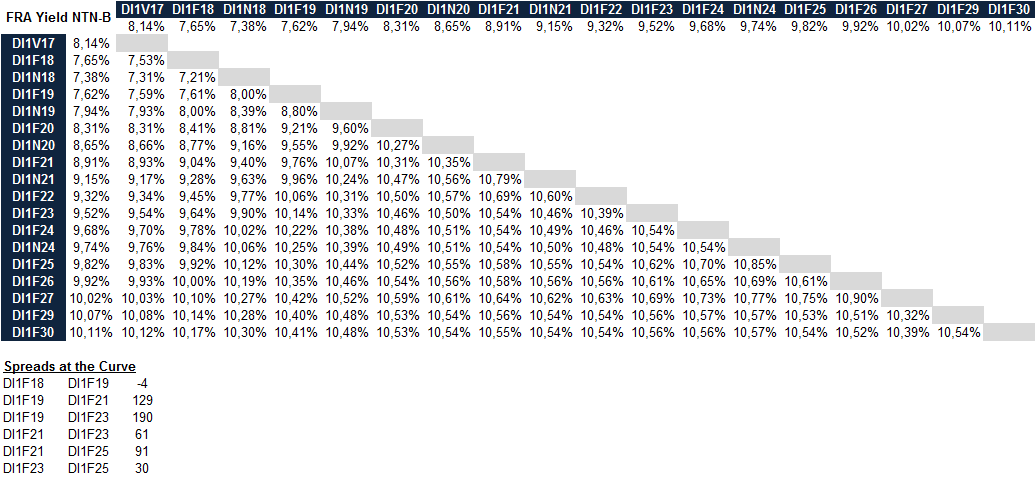
\includegraphics[angle=90,width=10.5cm]{images/FRA_DI.png}
\end{center}

\newpage


\section{Disclaimer}
\label{sec:org7cac1ed}
\smallsize
\begin{quote}
This report has been produced by Guide Investimentos S.A Corretora de
Valores solely for its recipients and should not be distributed
without previous consent from Guide Investimentos S.A.  Although this
report is based upon the most reliable public information, Guide
Investimentos makes no warranties of the reliability of such
information. This document is for informational purposes only and does
not constitute any tender to sell or buy financial
instruments. Information discussed herein is not suitable for all
investors and it does not aim at providing any trading strategy for
individual goals. Investors should have experience and knowledge of
the risks in FX/Fixed Income markets. Guide Investimentos S.A
Corretora de Valores has no obligation to update, revise or modify any
information contained herein. Guide Investimentos and its analysts
shall not be held responsible for any accidental incorrect
information, nor for investment decisions taken based upon the
information contained herein. Additional information discussed on this
report is available upon request.  Analysts each certify that the
views expressed in this report represent only personal views produced
independently, including with respect Guide Investimentos S.A
Corretora de Valores. This report should not be considered as research
report ("relat�rio de an�lise") for the purposes of the article 1 of
CVM Instruction NR 483. Opinions, estimates and projections contained
herein express the current judgment of the analysts build on the date
this report was released and therefore can be changed without
notice. Analysts do not accept any liability that incorrect use of
this report could cause, including financial losses. Upon accepting
this document, one should agree with all the above-mentioned
limitations
\end{quote}
\end{document}
